\chapter{Method}
\label{chap:method}

This chapter describes the DRIFT framework: the bitemporal substrate that every experimental condition shares, the pipeline that connects raw conversation to a judged answer, the seven forgetting policies compared, the metrics reported, and the statistical procedures used to test differences between policies. The organizing design principle, stated once here and referred to throughout the remainder of this thesis, is that the forgetting policy is the only component of the pipeline that is allowed to differ between experimental conditions. Everything upstream and downstream of the policy, including how a fact is extracted from text, how it is retrieved, how an answer is generated from it, and how that answer is judged, is identical across every condition. This is what licenses attributing any measured difference in outcome to the policy rather than to some other, uncontrolled, source of variation.

\section{The Substrate}
\label{sec:substrate}

Every fact stored by DRIFT is represented as a subject, predicate, object triple, carrying two independent timelines and a lifecycle marker. Table~\ref{tab:fact-fields} lists the fields and their meaning.

\begin{table}[H]
\centering
\caption{Fields carried by every fact in the bitemporal substrate.}
\label{tab:fact-fields}
\begin{tabular}{lp{4.3in}}
\toprule
Field & Meaning \\
\midrule
\texttt{t\_valid\_start} & When the fact became true of the world \\
\texttt{t\_invalid\_at} & When the fact stopped being true, null while current \\
\texttt{t\_ingested} & When the agent learned the fact \\
\texttt{t\_pruned} & When a policy removed the fact, null while retained \\
\texttt{provenance} & Which agent wrote the fact \\
\texttt{active} & False once the fact has been pruned \\
\bottomrule
\end{tabular}
\end{table}

The distinction between \texttt{t\_valid\_start} and \texttt{t\_ingested} is the defining property of a bitemporal system, as opposed to a system that records only a single timestamp per fact. A single timestamp cannot distinguish ``this became true on this date'' from ``I learned this on this date,'' and the two dates frequently differ: an agent may be told today about something that became true months ago, or an agent may need to reason about what it believed at a past point in time regardless of what has since turned out to be true. Recording both timelines separately, rather than collapsing them into one, is what allows the substrate to represent the full history of a fact's status without discarding information at the point of storage.

When a new fact arrives that shares its subject and predicate with an existing fact, and that predicate has been declared \emph{functional}, meaning it is understood to admit only one true object at a time, the previous fact's valid-time window is closed by setting its \texttt{t\_invalid\_at} field to the time of the new observation. Critically, this closing operation is \emph{non-destructive}: the superseded fact remains in memory, remains addressable, and remains retrievable by any downstream component that chooses to retrieve it. No fact is ever deleted or hidden as a direct consequence of a contradiction being detected. The only thing a contradiction does, on its own, is close a validity window.

This separation between detecting a contradiction and acting on it is the methodological core of the entire experimental design. It guarantees that the graph itself behaves identically under every experimental condition, regardless of which policy is active, because contradiction closing happens at the substrate layer, below and prior to any policy's involvement. The only thing that differs between conditions is what a policy subsequently chooses to do with a fact whose window has been closed: retain it and let it be retrieved, filter it out at retrieval time, or prune it outright. Any difference in outcome observed between two conditions can therefore be attributed to that choice, and to nothing else, because everything upstream of the policy is byte-for-byte identical between conditions.

\paragraph{The speech-act guard.} A practical safeguard is applied before contradiction detection runs. Predicates such as \emph{stated}, \emph{said}, \emph{mentioned}, and \emph{reported} are excluded from contradiction handling even in a configuration where every predicate has been declared functional. Without this exclusion, a degenerate extraction pattern in which every line of a session is extracted as \emph{speaker / stated / entire line} causes every fact to contradict the fact immediately before it, because every extracted triple shares the same subject and predicate and differs only in its object. This failure mode was measured directly during development: on a corpus whose true number of genuine contradictions is 133, a version of the substrate without the speech-act guard invalidated 379 of 380 facts. The failure is silent, in the sense that it produces a graph that looks superficially plausible, and it can resemble a legitimate policy result to someone inspecting only summary statistics rather than the underlying extraction. It is reported here because it is the kind of error that is easy to introduce and hard to notice after the fact.

\section{The Pipeline}
\label{sec:pipeline}

Figure~\ref{fig:architecture} shows the full pipeline that connects a raw session of conversation lines to a judged answer. Every experimental cell in this thesis executes the identical sequence of stages shown in the figure; the only stage that varies between cells is the policy, which is invoked at exactly three points.

\begin{figure}[H]
\centering
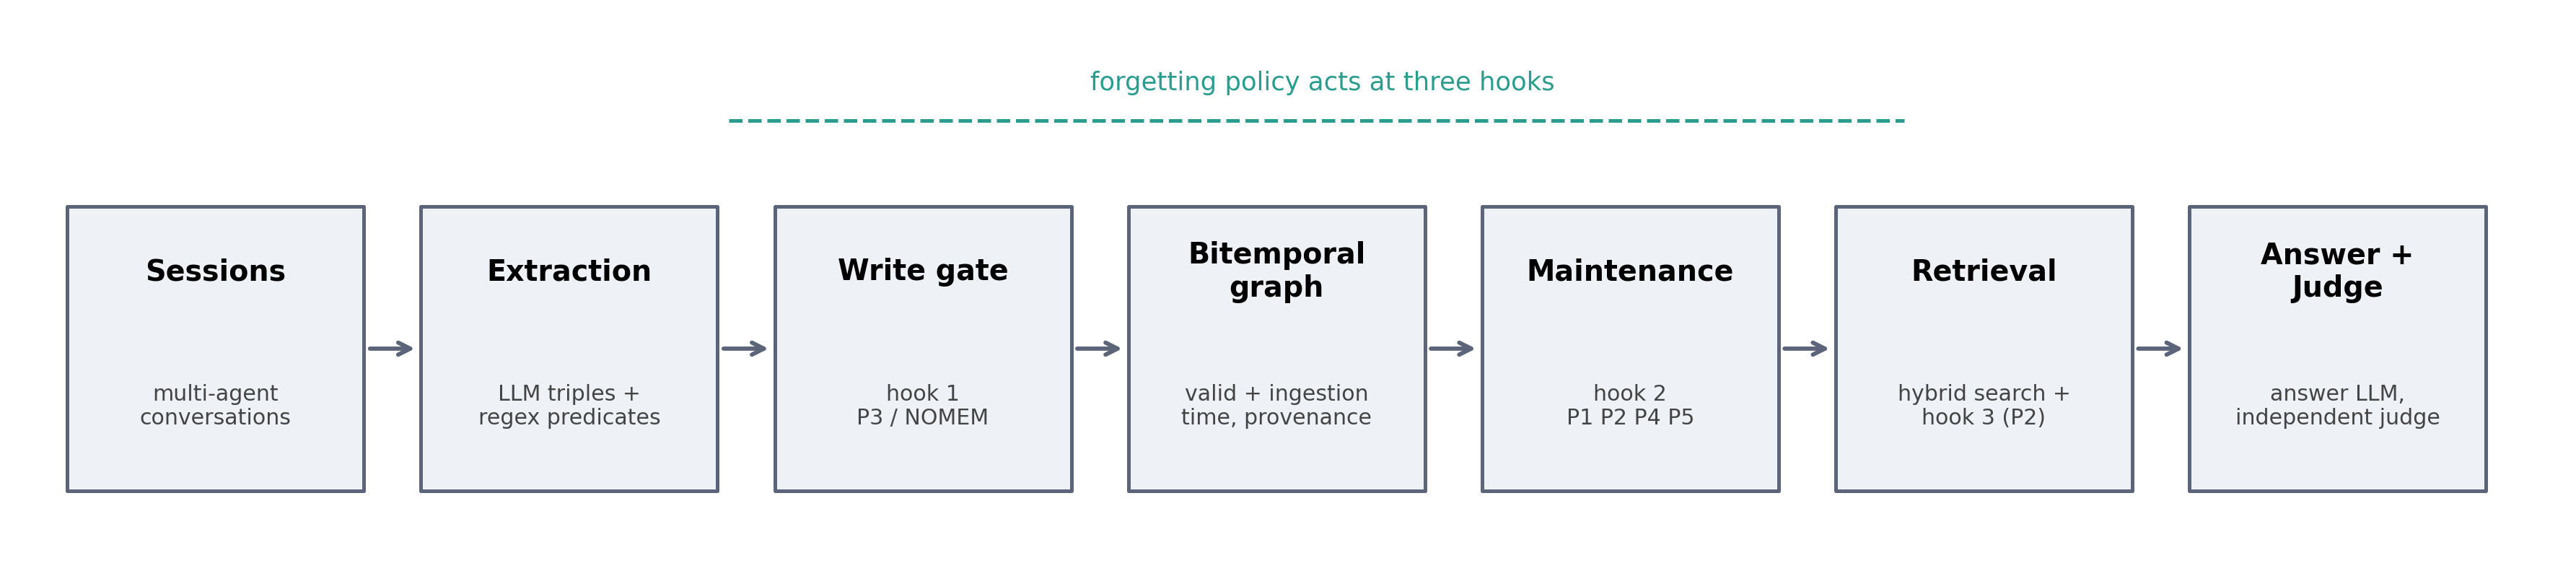
\includegraphics[width=0.85\textwidth]{figures/architecture.png}
\caption{The DRIFT pipeline. Session text is converted to facts, facts pass through the bitemporal substrate where contradictions on functional predicates close validity windows, a policy performs periodic maintenance, retrieval ranks candidate facts, a second policy hook filters or reranks what the answer model sees, and the answer is scored by an independent judge alongside a token-overlap metric.}
\label{fig:architecture}
\end{figure}

The stages, in order, are as follows. Session lines are converted into candidate facts by a language-model extraction step, backed by a deterministic regular-expression upgrade applied specifically to functional predicates, so that contradiction detection does not depend on the extractor happening to phrase two related facts identically. Each candidate fact is offered to the active policy's write hook, which may reject it outright before it ever enters the graph. Facts that are accepted enter the bitemporal knowledge graph, where a contradiction on a functional predicate closes the superseded fact's validity window in the non-destructive manner described in Section~\ref{sec:substrate}. After each session, the active policy's periodic-maintenance hook runs, which is where time-based pruning, grace-period pruning, language-model consolidation, or topology-based consolidation take place, depending on which policy is active. When a question is asked, retrieval ranks candidate facts by a fixed hybrid score combining cosine similarity, lexical overlap, and recency, weighted 0.6, 0.3, and 0.1 respectively, and returns the top $k = 25$ candidates. The active policy's retrieval hook then has the opportunity to filter or rerank this candidate set before it is handed to the answer model. The answer model produces a response, which is then scored twice: once by a large language model judge drawn from a different model family than the answer model, and once by a token-level F1 overlap metric that does not depend on a judge at all.

A policy is defined by exactly three hooks, shown in the interface below. Adding a new policy to the framework is a matter of subclassing this interface and registering the subclass; no other component of the pipeline, including the runner, the substrate, the model providers, or the analysis code, needs to be modified or even needs to be aware that a new policy exists.

\begin{verbatim}
class Policy:
    def on_write(self, fact, graph) -> bool:
        ...  # returning False rejects the write

    def after_session(self, graph, provider, now):
        ...  # periodic maintenance, run once per session

    def on_retrieve(self, facts, now) -> list:
        ...  # filter or rerank what the answer model sees
\end{verbatim}

\section{Policies Under Test}
\label{sec:policies}

Seven policies are compared, spanning a floor baseline, a ceiling baseline, and five distinct forgetting strategies. Table~\ref{tab:policies} summarizes each policy's mechanism and the hook or hooks it uses.

\begin{table}[H]
\centering
\caption{The seven policies compared in this thesis.}
\label{tab:policies}
\small
\begin{tabular}{lp{2.6cm}p{5.4cm}p{2.6cm}}
\toprule
ID & Name & Mechanism & Hooks used \\
\midrule
NOMEM & No memory & Retrieval returns nothing; a floor baseline & \texttt{on\_retrieve} \\
P0 & No forgetting & Append-only; nothing gated, pruned, or filtered; a ceiling baseline & none \\
P1 & TTL decay & Prune facts older than a fixed number of days by valid time & \texttt{after\_session} \\
P2 & Contradiction invalidation & Exclude superseded facts at retrieval time; prune after a seven-day grace period & \texttt{on\_retrieve}, \texttt{after\_session} \\
P3 & Novelty gate & Reject writes whose neighborhood cosine similarity exceeds a threshold of 0.9 & \texttt{on\_write} \\
P4 & LLM consolidation & Every third session, a language model decides which facts to keep or drop, plus a deterministic near-duplicate merge & \texttt{after\_session} \\
P5 & Topology consolidation & Resolve competing facts by structural corroboration count, deliberately denied access to valid time & \texttt{after\_session} \\
\bottomrule
\end{tabular}
\end{table}

\paragraph{NOMEM as a baseline.} The prompt given to the answer model instructs it to respond ``I don't know'' whenever memory does not contain the answer to a question. Under NOMEM, memory always fails to contain the answer, by construction, and the model's responses are almost entirely that refusal string, including in cases where the underlying language model plainly has the answer available from its own training. NOMEM therefore measures memory-gated answering behavior, not the model's parametric knowledge, and the gap between P0 and NOMEM should be read as the value memory adds under an explicit instruction to ground answers in memory rather than in general knowledge. A consequence worth stating plainly: NOMEM's staleness of exactly 0.000, reported in Chapter~\ref{chap:results}, is trivially achieved by refusing to answer at all, and staleness figures are only meaningfully comparable among policies that actually attempt an answer.

\paragraph{P5 as an ablation.} Policy P5 is not included because it is expected to perform well. It is included specifically to test whether the advantage of bitemporal reasoning comes from temporal information in particular, or merely from any form of graph-aware consolidation. P5 builds an entity co-occurrence graph from the same underlying facts P2 has access to, finds communities of related entities using label propagation, and within each community resolves competing facts sharing the same subject and predicate by retaining whichever candidate object is corroborated by the largest number of other facts elsewhere in memory. High-degree entities, meaning entities that participate in many facts, are protected from being pruned below a floor threshold. P5 has access to every structural signal P2 has access to, with the single exception of valid time.

\section{Metrics}
\label{sec:metrics}

Five quantities are reported for every experimental cell.

\paragraph{Accuracy.} A language model judge, drawn from a model family different from the answer model, returns a binary verdict of correct or incorrect against the gold answer for each question. Judges are drawn from a pool of three providers with automatic fallback between them; Section~\ref{sec:judge-audit} audits the consequences of this rotation for the reliability of the accuracy metric itself.

\paragraph{Staleness.} The fraction of answers that contain the superseded value for a question, computed as a case-insensitive substring test between the model's answer and the question's annotated \texttt{stale\_answer} field:

\begin{verbatim}
def staleness_hit(answer, stale_answer):
    if not stale_answer:
        return False
    return stale_answer.lower() in answer.lower()
\end{verbatim}

Staleness can only fire on questions that carry a \texttt{stale\_answer} annotation, which means a benchmark's annotation coverage places a hard upper bound on what this metric is capable of reporting for that benchmark. This is not a minor caveat; it is the subject of Section~\ref{sec:benchmark-selection}, and it is the source of a false result the author initially mistook for a finding before diagnosing its cause.

\paragraph{Token-F1.} Unigram overlap between the model's answer and the gold answer, reported alongside accuracy because it does not depend on a judge at all. It penalizes verbose answers, which is why the two answer models used in this thesis diverge sharply on this metric while agreeing closely on judge-scored accuracy; Section~\ref{sec:per-model} discusses this divergence and its implication for metric selection.

\paragraph{Cost.} The mean number of tokens consumed per question at answer time, together with the count of facts the policy retains as active in memory at the end of the run.

\paragraph{Retrieved-invalidated.} The mean number of facts appearing in a retrieval that have had their validity window closed by a contradiction. This is the mechanism variable underlying the staleness metric: it is exactly 0.00 for policy P2 by construction, because P2's retrieval hook filters such facts out before the answer model ever sees them, and it ranges from roughly 4.2 to 5.4 for the policies that do not filter on this basis.

\section{Statistics}
\label{sec:statistics}

Four statistical procedures are used throughout Chapter~\ref{chap:results}, chosen specifically because the design compares policies that are evaluated on the identical set of questions rather than on independent samples.

\begin{itemize}
\item \textbf{Bootstrap 95 percent confidence intervals}, computed by the percentile method with 5,000 resamples, reported for every accuracy and staleness figure.
\item \textbf{Paired McNemar exact test}, using the exact two-sided binomial distribution over discordant pairs, for comparing two policies on the same set of questions. Because every policy answers the identical question set, an unpaired test would overstate the significance of an observed difference by treating correlated outcomes as independent.
\item \textbf{Paired bootstrap on the per-question difference}, used to estimate effect sizes. This procedure is a stronger form of evidence than comparing two overlapping confidence intervals computed independently for each policy, and it is what allows a failure to reject a null hypothesis to be reported as a bounded equivalence claim rather than as an inconclusive result, a distinction developed at length in Section~\ref{sec:rq2}.
\item \textbf{Spearman's rank correlation}, computed on the policy rankings produced by each benchmark, used to quantify how well a ranking established on one benchmark generalizes to a second benchmark of different provenance.
\end{itemize}
